%!TEX root = ../notes.tex
\section{January 31, 2023}

\subsection{Properties of Functions}
We introduce some properties of functions:
\begin{definition}[Injectivity]
    A function $f: A\to B$ is \ul{injective} (one-to-one) if
    \[f(a_1) = f(a_2)\implies a_1 = a_2.\]
    ``No two elements in $A$ map to the same element in $B$.''
    \begin{center}
        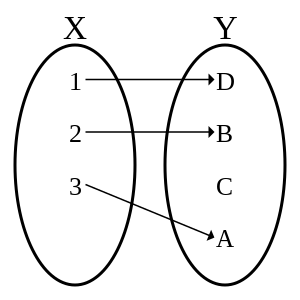
\includegraphics[width=0.2\linewidth]{images/injective.png}

        (Using $X$ and $Y$, injective but not surjective.)
    \end{center}
\end{definition}

\begin{definition}[Surjectivity]
    A function $f: A\to B$ is \ul{surjective} (onto) if
    \[\forall b\in B, \exists a\in A, \text{ s.t. }f(a) = b.\]
    ``Every element in $B$ has a preimage in $A$.''
    \begin{center}
        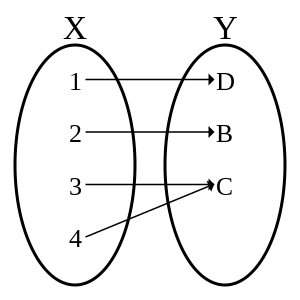
\includegraphics[width=0.2\linewidth]{images/surjective.png}

        (Using $X$ and $Y$, surjective but not injective.)
    \end{center}
\end{definition}

\begin{definition}[Functional Composition]
    Suppose $f: A\to B$ and $g: B\to C$ are functions, then $(g\circ f): A\to C$ with
    \[(g\circ f)(a) := g(f(a)).\]
\end{definition}

\begin{proposition}
    Let $f: A\to B$, $g: B\to C$ be functions, then if $f, g$ are both injective, then so is $(g\circ f)$.

    The same holds if they are surjective.
\end{proposition}
\begin{proof}[Proof of injective part]
    Let $a, a'\in A$ be such that
    \begin{align*}
        (g\circ f)(a) & = (g\circ f)(a') \\
        g(f(a))       & = g(f(a'))       \\
        \intertext{With $g$ injective, therefore}
        f(a)          & = f(a')
        \intertext{With $f$ injective, we then have}
        a             & = a'
    \end{align*}
    Therefore, $(g\circ f)$ is injective.
\end{proof}

\begin{proof}[Proof of surjective part]
    We want to show that $\forall c\in C$, $\exists a\in A$ such that $g(f(a)) = (g\circ f)(a) = c$.

    Since $g$ is surjective, $\exists b\in B$ s.t. $g(b) = c$.

    Since $f$ is surjective, $\exists a\in A$ such that $f(a) = b$.

    Now, plugging in, $g(f(a)) = g(b) = c$. Therefore, exists such a pre-image $a\in A$ for every $c\in C$ under $(g\circ f)$. Hence, $(g\circ f)$ is surjective.
\end{proof}

\begin{definition}[Bijectivity]
    If $f: A\to B$ is injective and surjective, we call $f$ a \ul{bijection}.
\end{definition}

\begin{theorem}[Existence of Inverse]
    Let $f: A\to B$, then $\exists f^{-1}: B\to A$ such that
    \begin{align*}
        f^{-1}\circ f = \mathrm{id}_A \\
        f\circ f^{-1} = \mathrm{id}_B
    \end{align*}
    where
    \begin{align*}
        \Id_A: A\to A, \quad \forall a\in A, \Id_A(a) = a \\
        \Id_B: B\to B, \quad \forall b\in B, \Id_B(b) = b
    \end{align*}
    if and only if $f$ is a bijection.
\end{theorem}
\begin{proof}
    ~\begin{description}
        \item[$\Longleftarrow$:] Suppose $f: A\to B$ is a bijection. Then, we define $f^{-1}\subset B\times A$ as
            \[f^{-1} = \{(b, a)\mid (a, b)\in f\}\]
            It's clear that this is a relation. We check that $f^{-1}$ is a function.

            That is, we need to check that $\forall b\in B$, there exists one and only one $a\in A$ such that $(b, a)\in f^{-1}$.

            In other words, taking the definition of $f^{-1}$, we have to check that $\forall b\in B$, $\exists!\footnote{$\exists!$ as `exists exactly one'.} a\in A$ such that $(a, b)\in f$. This is exactly $f$ being bijective.

            Let's now show that
            \begin{align}
                f^{-1}\circ f & = \Id_A \label{eq:inverse-1} \\
                f\circ f^{-1} & = \Id_B \label{eq:inverse-2}
            \end{align}

            Let's first show \cref{eq:inverse-1}, suffices to show $f^{-1}(f(a))\overset{?}{=}a, \forall a$.

            $\forall a\in A$, $\exists b\in B$ such that $f(a) = b$, so $(a, b)\in f$. By definition, $(b, a)\in f^{-1}$ so $f^{-1}(b) = a$. Then $f^{-1}(f(a)) = f^{-1}(b) = a$.

            We do \cref{eq:inverse-2} very similarly.

        \item[$\Longrightarrow$:] Suppose $f: A\to B$ and $g\footnote{We use $g$ to reduce confusion with $f^{-1}$}: B\to A$ such that $g\circ f = \Id_A$ and $f\circ g= \Id_B$. We show that $f$ is a bijection.

            We first show injectivity. Suppose $f(a_1) = f(a_2)$, applying $g$ on both sides gives
            \begin{align*}
                g(f(a_1))  & = g(f(a_2))  \\
                \Id_A(a_1) & = \Id_A(a_2) \\
                a_1        & = a_2
            \end{align*}
            This gives us injectivity.

            We then show surjectivity. Let $b\in B$, we claim $\exists a\in A$ such that $f(a) = b$. Take $a := g(b)$, then $f(a) = f(g(b)) = b$. We've found such an $a$ such that $f(a) = b$, giving us surjectivity.
    \end{description}
    In both directions, this gives us the bijection.
\end{proof}

\begin{remark}
    Let $f: A\to B$ be a bijection, with $A$ and $B$ finite. We have that $A$ has $n$ elements $\iff$ $B$ has $n$ elements. That is, $A$ and $B$ have equal cardinality.

    This extends to arguments on infinite sets too, like between $\ZZ$ and $\QQ$. $\QQ$ and $\RR$ or $\ZZ$ and $\RR$ have different cardinalities and hence don't have bijections.
\end{remark}

If $f: A\to B$ is not a bijection, we cannot define an inverse in the same way as we did before. But, we can consider the inverse image.

\begin{definition}[Inverse Image]
    Given function $f: A\to B$, $C\subseteq B$ we define the \ul{inverse image} of $C$ as
    \[f^{-1}(C) := \left\{ a\in A\mid f(a)\in C \right\}.\]
    ``The set of $a\in A$ that take me somewhere in $C$.''
\end{definition}

If $C = \{b\}$, we get all elements mapped to $b$. That is,
\[f^{-1}(\{b\}) = \left\{ a\in A\mid f(a) = b \right\}\]

\subsection{Cardinality}
\begin{definition}[Cardinality]
    If $A, B$ are sets, we say that $A$ and $B$ are equivalent ($A\simeq B)$ if there exists a bijective $f: A\to B$. This is an equivalence relation.

    The \ul{cardinality} of a set $A$ ($\#(A)$) is the equivalence class of $A$ under this relation:
    \[\#(A) := \{B\mid A\simeq B\}.\]
\end{definition}

\begin{remark}
    When $A$ is finite with $n$ elements, this is an abuse of notation. $\#(A)$ is the set of all sets with $n$ elements, or we also say the `cardinality' of $A$ is simply $n$.
\end{remark}

\begin{example}
    Consider $\ZZ$, the set of integers. Consider $2\ZZ$, the set of even integers. They belong to the same cardinality. Even though they are infinite sets, they are the `same level' of infinite\footnote{Even though we might think that $2\ZZ\subseteq \ZZ$.}.

    Specifically, we have bijection $f: \ZZ\to 2\ZZ$ with $x\mapsto 2x$.
\end{example}

\subsection{Natural Numbers}
We'll assume the Peano Axioms, which are the following:
\begin{enumerate}[A.]
    \item $\exists \NN$, an element $1\in \NN$.
    \item a function $s: \NN\to \NN$ satisfying
          \begin{enumerate}[(1)]
              \item $\forall n\in \NN, s(n) \neq 1$,
              \item $s$ is injective,
              \item if $\exists S$, such that $1\in S\subset \NN$, and $S$ satisfies that whenever $n\in S$, then $s(n)\in S$, this implies $S = \NN$.
          \end{enumerate}
\end{enumerate}

Why do we need condition (3)?
\begin{example}
    Picking the half integers
    \[\left\{\frac{n}{2}\mid n\in \NN\right\}\]
    satisfies the first two conditions but not the third.
\end{example}

$s$ is called the \emph{successor} function.

\begin{proposition}
    For every $n\in \NN$, $s(n)\neq n$.
\end{proposition}
\begin{proof}
    Let
    \[S = \left\{ n\in \NN\mid s(n) \neq n \right\}.\]
    Clearly, $1\in S$ by axiom (1). Suppose $n\in S$ for some $n$. We claim that $s(n)\in S$. By the injectivity of $s$, $s(n)\neq n$ so $s(s(n)) \neq s(n)$.

    By (3), $S = \NN$ which gives $s(n)\neq n, \forall n$. We can never loop when we keep applying $s$.
\end{proof}
\begin{definition}[Natural Number]
    We'll call $s(1) = 2, s(2) = 3, \dots$. These are the natural numbers.
\end{definition}